\documentclass[12pt]{beamer}
\usepackage{../Estilos/BeamerMAF}
\usetheme{Copenhagen}
\usecolortheme{wolverine}
%\useoutertheme{default}
\setbeamercovered{invisible}
% or whatever (possibly just delete it)
\setbeamertemplate{section in toc}[sections numbered]
\setbeamertemplate{subsection in toc}[subsections numbered]
\setbeamertemplate{subsection in toc}{\leavevmode\leftskip=3.2em\rlap{\hskip-2em\inserttocsectionnumber.\inserttocsubsectionnumber}\inserttocsubsection\par}
% \setbeamercolor{section in toc}{fg=blue}
% \setbeamercolor{subsection in toc}{fg=blue}
% \setbeamercolor{frametitle}{fg=blue}
\setbeamertemplate{caption}[numbered]

\setbeamertemplate{footline}
\beamertemplatenavigationsymbolsempty
\setbeamertemplate{headline}{}


\makeatletter
% \setbeamercolor{section in foot}{bg=gray!30, fg=black!90!orange}
% \setbeamercolor{subsection in foot}{bg=blue!30}
% \setbeamercolor{date in foot}{bg=black}
\setbeamertemplate{footline}
{
  \leavevmode%
  \hbox{%
  \begin{beamercolorbox}[wd=.333333\paperwidth,ht=2.25ex,dp=1ex,center]{section in foot}%
    \usebeamerfont{section in foot} \insertsection
  \end{beamercolorbox}%
  \begin{beamercolorbox}[wd=.333333\paperwidth,ht=2.25ex,dp=1ex,center]{subsection in foot}%
    \usebeamerfont{subsection in foot}  \insertsubsection
  \end{beamercolorbox}%
  \begin{beamercolorbox}[wd=.333333\paperwidth,ht=2.25ex,dp=1ex,right]{date in head/foot}%
    \usebeamerfont{date in head/foot} \insertshortdate{} \hspace*{2em}
    \insertframenumber{} / \inserttotalframenumber \hspace*{2ex} 
  \end{beamercolorbox}}%
  \vskip0pt%
}
\makeatother

\makeatletter
\patchcmd{\beamer@sectionintoc}{\vskip1.5em}{\vskip0.8em}{}{}
\makeatother

% %\newlength{\depthofsumsign}
% \setlength{\depthofsumsign}{\depthof{$\sum$}}
% \newcommand{\nsum}[1][1.4]{% only for \displaystyle
%     \mathop{%
%         \raisebox
%             {-#1\depthofsumsign+1\depthofsumsign}
%             {\scalebox
%                 {#1}
%                 {$\displaystyle\sum$}%
%             }
%     }
% }
% \def\scaleint#1{\vcenter{\hbox{\scaleto[3ex]{\displaystyle\int}{#1}}}}
% \def\scaleoint#1{\vcenter{\hbox{\scaleto[3ex]{\displaystyle\oint}{#1}}}}
% \def\bs{\mkern-12mu}


\makeatletter
\setbeamercolor{section in foot}{bg=cadetblue!20}
\setbeamercolor{subsection in foot}{bg=OliveGreen!30}
\makeatother

%\DeclareMathOperator\erf{Erf}
\DeclareMathOperator\erfc{erfc}


\date{18 de enero de 2022}

\title{\large{Transformada de Laplace}}
\author{M. en C. Gustavo Contreras Mayén}

\begin{document}
\maketitle
\fontsize{14}{14}\selectfont
\spanishdecimal{.}

\section*{Contenido}
\frame[allowframebreaks]{\tableofcontents[currentsection, hideallsubsections]}


%Referencia. Debnath - Chap. 2 Laplace Transform 3.9
\section{Definiciones}
\frame{\tableofcontents[currentsection, hideothersubsections]}
\subsection{La TL y su inversa}

\begin{frame}
\frametitle{La Transformada de Laplace}
Definimos la transformada de Laplace (TL) de una función continua en tramos de variable real $t$, definida en un semieje $t \geq 0$ como:
\pause
\begin{eqnarray}
\begin{aligned}
L \big[f(t); t \to p\big] &= \pause L \big[f(t)\big] = \pause F(p) = \pause \overline{f}(p) = \\[0.5em] \pause
&= \scaleint{6ex}_{\bs 0}^{\infty} f(t) \, \exp(-p \, t) \dd{t}
\end{aligned}
\label{eq:ecuacion_03_03}
\end{eqnarray}
\end{frame}
\begin{frame}
\frametitle{La TL inversa}
La transformada inversa de Laplace se define como:
\pause
\begin{eqnarray}
\begin{aligned}
f(t) &= \pause L^{-1} \big[\overline{f}(t); p \to t\big] = \pause L^{-1} \big[F(p)\big] = \\[0.5em] \pause
&= \dfrac{1}{2 \pi \, i} \scaleint{6ex}_{\bs \gamma-i \infty}^{\gamma+\infty} \exp(p \, t) \, \overline{f} (p) \, \dd{p}
\end{aligned}
\label{eq:ecuacion_03_04}
\end{eqnarray}
donde $\gamma = \Re{p} > 0$.
\end{frame}

\section{Uso de las propiedades de la TL}
\frame{\tableofcontents[currentsection, hideothersubsections]}
\subsection{Ejemplo 1}

\begin{frame}
\frametitle{Evaluación de la TL}
Evalúa la TL:
\pause
\begin{align*}
L \big[ \sin (t - a) \, H (t - a); t \to p  \big]
\end{align*}
\pause
Y con ese resultado, evalúa:
\pause
\begin{align*}
L \big[ \exp\big[ (t - a ) k \big] \sin (t - a) \, H (t - a); t \to p  \big]
\end{align*}
\end{frame}
\begin{frame}
\frametitle{Solución al Ejemplo 1}
Para resolver este ejemplo, debemos de ocupar el resultado de la TL:
\begin{eqnarray*}
\begin{aligned}
L \big[ \sin t ; t \to p  \big] &= \scaleint{6ex}_{\bs 0}^{\infty} \sin t \, \exp(-p \, t) \dd{t} = \\[0.5em] \pause
&= \dfrac{1}{p^{2} + 1}
\end{aligned}
\end{eqnarray*}
\end{frame}
\begin{frame}
\frametitle{Ocupando una propiedad de la TL}
Por el segundo teorema de desplazamiento de la TL:
\\
\bigskip
\pause
\noindent \textbf{Teorema: } Si la transformada de Laplace de $f(t)$ es $\overline{f}(p)$, entonces la transformada de Laplace de $f(t - a) \, H(t - a)$ es $\exp(-a \, p) \, \overline{f}(p)$.
\end{frame}
\begin{frame}
\frametitle{Ocupando el segundo teorema de desplazamiento}
Entonces se tiene que:
\begin{align*}
L \big[ \exp\big[ (t - a ) k \big] \sin (t - a) \, H (t - a) \big] = \dfrac{\exp (- p a)}{(1 + p^{2})}
\end{align*}
\end{frame}
\begin{frame}
\frametitle{Otra propiedad de la TL}
Ahora ocuparemos el primer teorema de desplazamiento para la TL:
\\
\bigskip
\pause
\noindent \textbf{Teorema: } Si la transformada de Laplace de $f(t)$ es $\overline{f}(p)$, entonces la transformada de Laplace de $\exp(a \, t)$ es $\overline{f}(p - a)$.
\end{frame}
\begin{frame}
\frametitle{Resultado del ejercicio}
Al ocupar el primer teorema del desplazamiento, llegamos al resultado:
\pause
\begin{eqnarray*}
\begin{aligned}
&L \big[ \exp\big[k (t - a) \big] \, \sin (t - a) \, H (t - a); t \to p  \big] = \\[0.5em]
&= \dfrac{\exp\big[ -(p - k) \big]}{\big[ 1 + (p - k)^{2} \big]}
\end{aligned}
\end{eqnarray*}
\end{frame}

\subsection{Ejemplo 2}

\begin{frame}
\frametitle{Enunciado del ejemplo}
Evalúa:
\pause
\begin{align*}
L \big[ \sinh bt; t \to p \big]
\end{align*}
\pause
Para luego obtener:
\pause
\begin{align*}
L \big[ \exp (a t) \, \sinh bt; t \to p \big]
\end{align*}    
\end{frame}
\begin{frame}
\frametitle{Solución}
Nuevamente nos apoyamos en un resultado de la TL de la función $\sinh t$:
\pause
\begin{eqnarray*}
\begin{aligned}
L \big[ \sinh t ; t \to p \big] &= \scaleint{6ex}_{\bs 0}^{\infty} \sinh t \, \exp(-p \, t) \dd{t} = \\[0.5em] \pause
&= \dfrac{1}{p^{2} - 1}
\end{aligned}
\end{eqnarray*}
\end{frame}
\begin{frame}
\frametitle{Usando otra propiedad de la TL}
Ocuparemos la propiedad de cambio de escala de la TL:
\\
\bigskip
\pause
\noindent \textbf{Teorema: } Si:
\begin{align*}
L \big[f(t); t \to p\big] &= \overline{f} (p)
\end{align*}
Entonces
\begin{align*}
L \big[f(a \, t); t \to p\big] &= \dfrac{1}{a}\overline{f} \left(\dfrac{p}{a}\right)
\end{align*}
\end{frame}
\begin{frame}
\frametitle{Resultado de la TL}
Luego de ocupar la propiedad de cambio de escala, tenemos que la TL es:
\pause
\begin{align*}
L \big[ \sinh b t ; t \to p \big] = \dfrac{b}{p^{2} - b^{2}}
\end{align*}
\end{frame}
\begin{frame}
\frametitle{Respuesta al ejemplo}
El resultado final del ejercicio es:
\pause
\begin{align*}
L \big[ \exp (a t) \, \sinh bt; t \to p \big] = \dfrac{b}{(p - a)^{2} + b^{2}}
\end{align*}
\end{frame}

\subsection{Ejemplo 3}

\begin{frame}
\frametitle{Enunciado del ejemplo}
Evalúa la TL:
\pause
\begin{align*}
L \big[ \exp (a t) \, \cos bt; t \to p \big]
\end{align*}
\pause
Con ese resultado, obtén:
\pause
\begin{align*}
L \big[ \exp\big[ a(t - c) \, \cos b (t - c) \, H (t - c); t \to p \big]
\end{align*}
\end{frame}
\begin{frame}
\frametitle{Resultado de utilidad}
Como hemos visto en los ejercicios previos, cuando se tiene una función que involucra a otras \enquote{funciones conocidas}, de las que es necesario contar con su TL, \pause es conveniente ocupar las TL de esas funciones ya sea en una lista o tabla.
\end{frame}
\begin{frame}
\frametitle{Resultado de utilidad}
En este caso, se requiere conocer el valor de la TL de:
\pause
\begin{align*}
L \big[ \cos b t; t \to p \big] = \dfrac{p}{p^{2} + b^{2}}
\end{align*}    
\end{frame}
\begin{frame}
\frametitle{Ocupando las respectivas propiedades}
Así mismo, se procede a ocupar las propiedades de la TL que sean las pertinentes, de esta manera se simplifica el trabajo para obtener la solución.
\end{frame}
\begin{frame}
\frametitle{Avanzando en la solución}
Al ocupar el teorema de desplazamiento:
\pause
\begin{align*}
L \big[ \exp(a t) \, \cos b t; t \to p \big] = \dfrac{p - a}{(p - a)^{2} + b^{2}}
\end{align*}
\end{frame}
\begin{frame}
\frametitle{Solución al ejercicio}
Al ocupar ahora otra de las propiedades de la TL, se llega al resultado final del ejercicio:
\pause
\begin{eqnarray*}
\begin{aligned}
&L \big[ \exp\big[ a(t - c) \, \cos b (t - c) \, H (t - c); t \to p \big] = \\[0.5em]
&= \exp (- p c) \, \dfrac{(p - a)}{(p - a)^{2} + b^{2}}
\end{aligned}
\end{eqnarray*}
\end{frame}

\subsection{Ejemplo 4}

\begin{frame}
\frametitle{Enunciado del ejemplo 4}
Evalúa las siguientes TL:
\pause
\setbeamercolor{item projected}{bg=blue!70!black,fg=yellow}
\setbeamertemplate{enumerate items}[circle]
\begin{enumerate}[<+->]
\item $L \big[ t \, H(t - 1); t \to p \big]$
\item $L \big[ H(t - 1) \, \cos a t; t \to p \big]$
\end{enumerate}
\end{frame}
\begin{frame}
\frametitle{Resultado para ambos incisos}
De la definición de:
\pause
\begin{eqnarray*}
\begin{aligned}
&L \big[ f(t) \, H (t - a); t \to p \big] = \scaleint{6ex}_{\bs a}^{\infty} \exp(- p t) \, f(t) \dd{t} = \\[0.5em] \pause
&=  \scaleint{6ex}_{\bs 0}^{\infty} \exp\big[ - p (u {+} a) \big] \, f(u {+} a) \dd{u} = \\[0.5em] \pause
&= \exp(- p a) \scaleint{6ex}_{\bs 0}^{\infty} \exp(- p u) \, f(u {+} a) \dd{u} = \\[0.5em] \pause
&= \exp(- p a) \, L \big[ f (t {+} a); t \to p \big]
\end{aligned}
\end{eqnarray*}
\end{frame}
\begin{frame}
\frametitle{Ocupando el resultado anterior}
Para resolver los dos incisos del ejercicio, ocuparemos el resultado que se obtuvo:
\pause
\begin{align*}
L \big[ f(t) \, H (t{-} a) \big] = \exp(- p \, a) \, L \big[ f (t {+} a); t \to p \big]    
\end{align*}
\end{frame}
\begin{frame}
\frametitle{Resolviendo el inciso i)}
Tenemos entonces que:
\pause
\begin{eqnarray*}
\begin{aligned}
&L \big[ t \, H(t {-} 1); t \to p \big] = \scaleint{6ex}_{1}^{\infty} \exp(- p t) \, t \dd{t} = \hspace{1cm} a = 1 \\[0.5em]
&= e^{-p} \scaleint{6ex}_{0}^{\infty} \exp(- p u) \, (t + 1) \dd{t} = \\[0.5em] \pause
&= e^{-p} \bigg[ \dfrac{1}{p^{2}} + \dfrac{1}{p} \bigg] = \pause \dfrac{p + 1}{p^{2}} \, e^{-p}
\end{aligned}
\end{eqnarray*}
\end{frame}
\begin{frame}
\frametitle{Resolviendo el inciso ii)}
Tenemos ahora que:
\pause
\begin{eqnarray*}
\begin{aligned}
&L \big[ H(t {-} 1) \, \cos a t \big] = \exp(- p) \, L \big[ \cos a (t + 1) \big] = \\[0.5em] \pause
&= e^{-p} \, L \big[ \cos a t \cdot \cos a - \sin a t \cdot \sin a \big] = \\[0.5em] \pause
&= \dfrac{e^{-p}}{p^{2} + 1} \, \big[ p \cos a - a \sin a \big]
\end{aligned}
\end{eqnarray*}
\end{frame}

% \subsection{Otra propiedad}

% \begin{frame}
% \frametitle{Una propiedad importante}
% Dentro de la lista de propiedades de la TL que se mencionan en las notas de trabajo, hay que agregar la siguiente:
% \\
% \bigskip
% \pause
% \noindent \textbf{Teorema: } Si la TL de una función continua en partes $f(t)$ es $\overline{f}(p)$, entonces la TL de:
% \pause
% \begin{align*}
% L \big[ t^{n} \, f(t); t \to p \big] = (-1)^{n} \, \dv[n]{\overline{f}(p)}{p}
% \end{align*}
% con $n$ un entero positivo.
% \end{frame}

\section{La TL de algunas funciones relevantes}
\frame{\tableofcontents[currentsection, hideothersubsections]}
\subsection{La función de Heaviside}

\begin{frame}
\frametitle{La conocida función $H (t)$}
Ya se presentó la función de Heaviside o de paso unitario, que está definida por:
\pause
\begin{align*}
H(t) = \begin{cases}
0, & t < 0 \\
1, & t > 0
\end{cases}
\end{align*}
\end{frame}
\begin{frame}
\frametitle{La función de paso unitario}
Esto generalmente se conoce como \enquote{función unitaria de Heaviside}.
\\
\bigskip
\pause
Cabe señalar además que cualquier función escalonada $f(t)$ siempre se puede expresar como una combinación de diferentes funciones de Heaviside.
\end{frame}
\begin{frame}
\frametitle{Combinación de funciones}
Por ejemplo, definamos una función escalonada mediante la relación:
\pause
\begin{align*}
f (t) = \begin{cases}
g (t), & 0 < t < a \\
k, & a < t < b \\
0, & t > b
\end{cases}
\end{align*}    
\end{frame}
\begin{frame}
\frametitle{Modificando la expresión}
La función $f (t)$ se puede escribir como:
\pause
\begin{align*}
f(t) = g(t) \, H (a - t) + k \big[ H (t - a) - H (t - b) \big]
\end{align*}
\end{frame}
\begin{frame}
\frametitle{La TL de $H (t)$}
Calculamos la TL de la función de paso unitario de Heaviside:
\pause
\begin{eqnarray*}
\begin{aligned}
L \big[ H (t) \big] &= \scaleint{6ex}_{\bs 0}^{\infty} H (t) \, \exp(- p t) \dd{t} = \\[0.5em]
&= \scaleint{6ex}_{\bs 0}^{\infty} 1 \cdot \exp(- p t) \dd{t} = \\[0.5em]
&= \dfrac{1}{p}
\end{aligned}
\end{eqnarray*}
\end{frame}
\begin{frame}
\frametitle{La TL inversa de $H (t)$}
Entonces tenemos que la TL inversa es:
\pause
\begin{align*}
L^{-1} \bigg[ \dfrac{1}{p} \bigg] = H (t)
\end{align*}
\end{frame}

\subsection{La función delta de Dirac}

\begin{frame}
\frametitle{La delta de Dirac}
Un problema que surge en la práctica es encontrar la transformada de Laplace inversa de la función unitaria o $H(t)$.
\\
\bigskip
\pause
Se presenta una caso similar en la función de impulso unitario $\delta (t)$.
\end{frame}
\begin{frame}
\frametitle{La delta de Dirac}
Dirac lo introdujo como $\delta (t)$ que actúa por un período de tiempo muy corto $\tau$ con un impulso finito $1$ que satisface las relaciones:
\pause
\begin{eqnarray}
\delta (t) &=& 0 \hspace{1.3cm} \mbox{para  } t \neq 0 \label{eq:ecuacion_03_25} \\[0.5em] \pause
\scaleint{6ex}_{\bs - \infty}^{\infty} \delta (t) \dd{t} &=& \scaleint{6ex}_{\bs 0}^{\tau} \delta (t) \dd{t} = 1 \label{eq:ecuacion_03_26}
\end{eqnarray}
\end{frame}
\begin{frame}
\frametitle{Sobre la delta de Dirac}
En el análisis matemático, dicha función es diferente a las funciones \enquote{ordinarias} y ocupar dicha función a veces conduce a inconsistencias en el análisis.
\\
\bigskip
\pause
Por ello, Dirac lo calificó como una \enquote{función impropia}.
\end{frame}
\begin{frame}
\frametitle{Sobre la delta de Dirac}
Puede usarse sólo cuando no se produzcan inconsistencias en el análisis.
\\
\bigskip
\pause
Así, formalmente tal función puede ser utilizada en el análisis clásico sin buscar rigor en el tratamiento.
\end{frame}
\begin{frame}
\frametitle{Sobre la delta de Dirac}
Las ecuaciones (\ref{eq:ecuacion_03_25}) y (\ref{eq:ecuacion_03_26}) anteriores no muestran una imagen clara de la $\delta (t)$.
\\
\bigskip
\pause
Dado que la variación precisa de $\delta (t)$ con $t$ en el intervalo no es un tema importante, pero su efecto es el punto de estudio, podemos usarlo correctamente suponiendo que no tiene oscilaciones bruscas e innecesarias en la vecindad de $t = 0$.
\end{frame}
\begin{frame}
\frametitle{Reescribiedo la $\delta (t)$}
Si reescribimos la función de paso $\delta_{\epsilon} (t)$ por:
\pause
\begin{align}
\delta_{\epsilon} (t) = \begin{cases}
0, & t < 0 \\
\dfrac{1}{\epsilon}, & 0 < t < \epsilon \\
0, & t > \epsilon
\end{cases}
\label{eq:ecuacion_03_27}
\end{align}
\end{frame}
\begin{frame}
\frametitle{El comportamiento de $\delta_{\epsilon} (t)$}
Entonces:
\pause
\begin{align}
\scaleint{6ex}_{\bs - \infty}^{\infty} \delta_{\epsilon} (t) \dd{t} = \scaleint{6ex}_{\bs 0}^{\epsilon} \dfrac{1}{\epsilon} \dd{t} = 1
\label{eq:ecuacion_03_28}
\end{align}
\pause
resulta que:
\pause
\begin{align}
\lim_{\epsilon \to 0} \delta_{\epsilon} (t) = \delta (t)
\label{eq:ecuacion_03_29}
\end{align}
como se definió en las ecs. (\ref{eq:ecuacion_03_25}) y (\ref{eq:ecuacion_03_26}).
\end{frame}
\begin{frame}
\frametitle{Ocupando la $\delta_{\epsilon} (t)$}
Si $f(t)$ es una función continua en la vecindad de $t = 0$, entonces:
\pause
\begin{eqnarray*}
\begin{aligned}
&\scaleint{6ex}_{\bs - \infty}^{\infty} \delta_{\epsilon} (t) \, f(t) \dd{t} = \scaleint{6ex}_{\bs 0}^{\epsilon} \delta_{\epsilon} (t) \, f(t) \dd{t} = \\[0.5em] \pause
&=\dfrac{1}{\epsilon} \scaleint{6ex}_{\bs 0}^{\epsilon} f(t) \dd{t} = \\[0.5em] \pause
&= \dfrac{f(\theta \epsilon)}{\epsilon} \scaleint{6ex}_{\bs 0}^{\epsilon} \dd{t} = \pause f (\theta \epsilon) \hspace{1cm} 0 < \theta < 1
\end{aligned}
\end{eqnarray*}
por el teorema del valor medio.
\end{frame}
\begin{frame}
\frametitle{Ajustando la función}
Por lo que:
\pause
\begin{align*}
\scaleint{6ex}_{\bs - \infty}^{\infty} f(t) \, \delta_{\epsilon} (t) \dd{t} = f (\theta \, \epsilon) \hspace{1.3cm} 0 < \theta < 1
\end{align*}
\pause
Ahora, al hacer que $\epsilon \to 0$, se obtiene:
\begin{align}
\scaleint{6ex}_{\bs - \infty}^{\infty} f(t) \, \delta (t) \dd{t} = f (0)
\label{eq:ecuacion_03_30}
\end{align}
\end{frame}
\begin{frame}
\frametitle{Expresión general}
De manera general, hacemos que:
\pause
\begin{eqnarray}
\begin{aligned}[b]
\scaleint{6ex}_{\bs - \infty}^{\infty} &f(\xi) \, \delta (\xi - a) \dd{\xi} = \\[0.5em] \pause
&= \scaleint{6ex}_{\bs - \infty}^{\infty} f(t + a) \, \delta \dd{t} =  \hspace{0.6cm} \mbox{con  } \xi - a = t \\[0.5em] \pause
&= f(0 + a) = \\[0.5em] \pause
&= f(a)
\end{aligned}
\label{eq:ecuacion_03_31}
\end{eqnarray}
\end{frame}
\begin{frame}
\frametitle{Utilidad del resultado}
Este es un resultado importante que puede usarse formalmente en el análisis siempre que no surja confusión.
\end{frame}
\begin{frame}
\frametitle{La TL de la $\delta (t)$}
La transformada de Laplace de $\delta (t)$ se da entonces por definición:
\pause
\begin{eqnarray}
\begin{aligned}[b]
L \big[ \delta (t); t \to p \big] &= \scaleint{6ex}_{\bs 0}^{\infty} \exp(- p t) \, \delta (t) \dd{t} = \\[0.5em] \pause
&= \exp( p \cdot 0) = \\[0.5em] \pause
&= 1 = \pause H (t) \hspace{1.3cm} t > 0
\end{aligned}
\label{eq:ecuacion_03_32}
\end{eqnarray}
\end{frame}
\begin{frame}
\frametitle{Conclusión}
Entonces tenemos que la TL:
\pause
\begin{align*}
L \big[ \delta (t); t \to p \big] = H (T)
\end{align*}
\pause
mientras que la TL inversa es:
\pause
\begin{align}
L^{-1} \big[ H (t) \big] = \delta (t)
\label{eq:ecuacion_03_33}
\end{align}
\end{frame}

\subsection{La función de error}

\begin{frame}
\frametitle{Definiendo la función de error}
La \textcolor{blue}{función de error} $\erf \, (t)$ se define como:
\pause
\begin{align*}
\erf \, (t) = \dfrac{2}{\sqrt{\pi}} \scaleint{6ex}_{0}^{t} \exp\big(-x^{2} \big) dd{x}
\end{align*}
\end{frame}
\begin{frame}
\frametitle{Gráfica de $\erf \, (t)$}
\begin{figure}
    \centering
    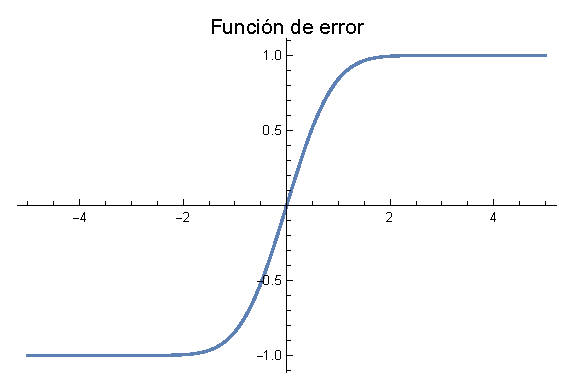
\includegraphics[scale=1]{Imagenes/Plot_Funcion_Error_01.eps}
\end{figure}
\end{frame}
\begin{frame}
\frametitle{Otra función de error}
La función complementaria de error $\erfc \, (t)$ es:
\pause
\begin{eqnarray}
\begin{aligned}[b]
&\erfc \, (t) = \dfrac{2}{\sqrt{\pi}} \scaleint{6ex}_{t}^{\infty} \exp^{-x^{2}} \dd{x} = \\[0.5em] \pause
&= 1 - \dfrac{2}{\sqrt{\pi}} \scaleint{6ex}_{0}^{t} \exp^{-x^{2}} \dd{x} = \pause 1 - \erf (t)
\end{aligned}
\label{eq:ecuacion_03_38}
\end{eqnarray}
ya que:
\begin{align*}
\dfrac{2}{\sqrt{\pi}} \scaleint{6ex}_{0}^{\infty} \exp\big(-x^{2} \big) \dd{x} = 1
\end{align*}
ocupando la función Gamma $\Gamma (x)$.
\end{frame}
\begin{frame}
\frametitle{Gráfica de $\erfc \, (t)$}
\begin{figure}
    \centering
    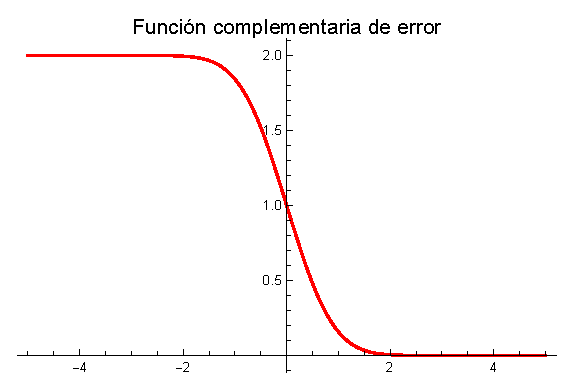
\includegraphics[scale=1]{Imagenes/Plot_Funcion_Error_02.eps}
\end{figure}
\end{frame}
\begin{frame}
\frametitle{Obteniendo la TL}
Por lo tanto, al evaluar la TL de $\erf \, (t)$, de la misma manera se puede evaluar fácilmente la TL de $\erfc \, (t)$.
\end{frame}
\begin{frame}
\frametitle{Procedimiento para las TL}
Para simplificar relativamente los pasos de evaluación, evaluamos la TL de $\erf \, \big( \sqrt{t} \big)$ en lugar de $\erf \,(t)$ con los siguientes pasos.
\end{frame}
\begin{frame}
\frametitle{Procedimiento para las TL}
Sabemos que:
\pause
\begin{eqnarray*}
\begin{aligned}
\erf \, \big( \sqrt{t} \big) &= \dfrac{2}{\sqrt{\pi}} \scaleint{6ex}_{\bs 0}^{\sqrt{t}} e^{-x^{2}} \dd{x} = \\[0.5em] \pause
&= \dfrac{2}{\sqrt{\pi}} \scaleint{6ex}_{\bs 0}^{\sqrt{t}} \bigg[ 1 - x^{2} + \dfrac{x^{2}}{2!} - \dfrac{x^{6}}{3!} + \cdots \bigg] = \\[0.5em] \pause
&= \dfrac{2}{\sqrt{\pi}} \bigg[ t^{\frac{1}{2}} - \dfrac{t^{\frac{3}{2}}}{3} + \dfrac{t^{\frac{5}{2}}}{5 \cdot 2!} - \dfrac{t^{\frac{7}{2}}}{7 \cdot 3!} + \cdots \bigg]
\end{aligned}
\end{eqnarray*}
\end{frame}
\begin{frame}
\frametitle{Obteniendo la TL}
Por lo tanto:
\pause
\begin{eqnarray*}
\begin{aligned}
&L \big[ \erf \, (\sqrt{t}) \big] = \dfrac{2}{\sqrt{\pi}} \bigg[ \dfrac{\Gamma (3/2)}{p^{\frac{3}{2}}} - \dfrac{\Gamma (5/2)}{3 \cdot p^{\frac{5}{2}}} + \dfrac{\Gamma (7/2)}{5 \cdot 2! \cdot p^{\frac{7}{2}}} + \\[0.5em]
&- \dfrac{\Gamma (9/2)}{7 \cdot 3! \cdot p^{\frac{9}{2}}} + \cdots \bigg] = \\[0.5em] \pause
&= \dfrac{1}{p^{\frac{3}{2}}} \bigg[ 1 - \dfrac{1}{2} \cdot \dfrac{1}{p} + \dfrac{1 \cdot 3}{2 \cdot 4} \cdot \dfrac{1}{p^{2}} - \dfrac{1 \cdot 3 \cdot 5}{2 \cdot 4 \cdot 6} \cdot \dfrac{1}{p^{3}} + \cdots \bigg]
\end{aligned}
\end{eqnarray*}
\end{frame}
\begin{frame}
\frametitle{Obteniendo la TL}
\begin{eqnarray}
\begin{aligned}[b]
L \big[ \erf \, (\sqrt{t}) \big] &= \dfrac{1}{p^{\frac{3}{2}}} \, \bigg( 1 + \dfrac{1}{p} \bigg)^{-\frac{1}{2}} = \\[0.5em] \pause
&= \dfrac{1}{p \, (p + 1)^{\frac{1}{2}}}
\end{aligned}
\label{eq:ecuacion_03_39}
\end{eqnarray}
\end{frame}
\begin{frame}
\frametitle{La Tl de $\erfc (\sqrt{t})$}
Por lo tanto:
\pause
\begin{eqnarray}
\begin{aligned}[b]
L \big[ \erfc \, (\sqrt{t}) \big] &= \pause L \big[ 1 - \erf \, (\sqrt{t}) \big] = \\[0.5em] \pause
&= \dfrac{1}{p} - \dfrac{1}{p \, (p + 1)^{\frac{1}{2}}} = \\[0.5em] \pause
&= \dfrac{(p + 1)^{\frac{1}{2}} - 1}{p (p + 1)^{\frac{1}{2}}}
\end{aligned}
\label{eq:ecuacion_03_40}
\end{eqnarray}
\end{frame}


\end{document}